\title{Multiplexor 6:1}
\date{2024-08-31}
\author{Daniel Josué Rodríguez Agraz}
\documentclass[9pt,technote]{IEEEtran}
\usepackage{filecontents,lipsum}
\usepackage[noadjust]{cite}
\usepackage{graphicx}
\usepackage{footmisc}
\usepackage{listings}
\usepackage{subcaption}
\usepackage{fancyhdr}
\usepackage{url}
\usepackage{hyperref}
\usepackage{array}
\hypersetup{
	colorlinks=true,
	linkcolor=black,
	urlcolor=blue,
	citecolor=black
}
%\usepackage[a4paper, total={6in, 10in}]{geometry}


\begin{document}
	
	\maketitle
	
	\section*{Objetivos}
	\begin{itemize}[]
	\item Describir el hardware de un multiplexor 6:1 utilizando la herramienta Questasim y realizar la verificación con distintos casos.
	\item Desarrollar un testbench para la verificación el circuito.
	\end{itemize}


	\section*{Introducción}
	Un multiplexor (MUX) es un dispositivo que permite dirigir la información digital procedente de diversas fuentes a una única línea para ser transmitida a través de dicha línea a un destino común. El multiplexor básico posee varias líneas de entrada de datos y una única línea de salida. También posee
	entradas de selección de datos, que permiten conmutar los datos digitales provenientes de cualquier entrada hacia la línea de salida. A los multiplexores también se les conoce como selectores de datos. \cite{floyd_fundamentos_nodate}
	
	La selección de una línea de entrada se controla con un conjunto de líneas de selección. Normalmente, hay $2^n$ líneas de entrada y $n$ líneas de selección cuyas combinaciones de bits determinan cuál entrada es seleccionada.\cite{mano_digital_2002}
	
	Un multiplexor de 6 líneas a 1 conecta una de seis fuentes a un destino común como se muestra en la figura \ref{fig:MUX6:1}. El circuito tiene seis líneas de entrada de datos, una línea de salida y una línea de selección S.
	
	\begin{figure}[htb]
		\centering
		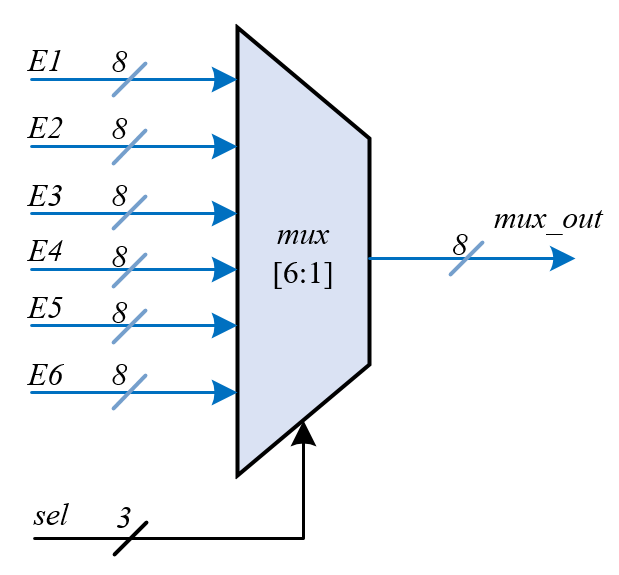
\includegraphics[scale=.3]{MUX61.png}
		\caption{Multiplexor de 6 lineas a 1.}
		\label{fig:MUX6:1}
	\end{figure}
		
	Como se muestra en la tabla \ref{Tabla:MUX6_VAL:1} los valores a la salida del multiplexor están directamente relacionados con el valor binario de la entrada de selección.
	
	
	
	\begin{table}[htb]
		\centering
		\begin{tabular}{|c|c|c|c|} 
			\hline
			Sel[2] & Sel[1] & Sel[0] & Output \\ [0.5ex] 
			\hline\hline
			0 & 0 & 0 & E1 \\ 
			\hline
			0 & 0 & 1 & E2 \\
			\hline
			0 & 1 & 0 & E3 \\
			\hline
			0 & 1 & 1 & E4 \\
			\hline
			1 & 0 & 0 & E5 \\
			\hline
			1 & 0 & 1 & E6 \\
			\hline
			1 & 1 & 0 & 0 \\
			\hline
			1 & 1 & 1 & 0 \\ [1ex] 
			\hline
		\end{tabular}
		\caption{Selección de datos de un multiplexor de 6 entradas y 1 salida.}
		\label{Tabla:MUX6_VAL:1}
	\end{table}
	
	En este trabajo se realizó la descripción de hardware y la verificación de un multiplexor 6:1 de 8 bits utilizando Questasim en lenguaje SystemVerilog. El objetivo principal fue diseñar y comprobar el correcto funcionamiento del multiplexor describiendo 14 casos con distintos valores y verificando los resultados a la salida. Tras la verificación, se comprobó que la salida era la esperada ante cambios en las entradas y en el selector, por lo que se pudo comprobar que la descripción era correcta dentro de esos casos.
	

	
	\section*{Desarrollo}
	% Desarrollo del proyecto.
	Para el desarrollo de este proyecto, se utilizó el lenguaje de descripción de hardware SystemVerilog en la herramienta Questasim. A continuación, se detallan los pasos seguidos:
	
	\subsection{Descripción del Hardware}
	Se describe el multiplexor 6:1 en SystemVerilog. Este toma seis entradas de 8 bits y las envía a una única salida de 8 bits, dependiendo de la señal de selección. La señal de selección consta de tres bits, que permiten seleccionar una de las seis entradas. Para lograr esto, se hizo uso de la sentencia `case` del propio lenguaje, como se muestra en el código a continuación.
	
	\begin{lstlisting}[language=Verilog, 
	caption={Descripción del multiplexor 6:1 en SystemVerilog}, 
	label={code:6to1mux}]
  module MUX6(
  input wire [7:0] E1,E2,E3,E4,E5,E6,
  input wire [2:0] sel,
  output reg [7:0] salida
  );

  always@(*) 
  begin
	case(sel)
	  3'b000: salida = E1;
	  3'b001: salida = E2;
	  3'b010: salida = E3;
	  3'b011: salida = E4;
	  3'b100: salida = E5;
	  3'b101: salida = E6;
	 default: salida = 8'h00;
	endcase
  end
	
  endmodule
	
	\end{lstlisting}
	
	\subsection{Verificación}
	En systemverilog, se crea un código de verificación, dónde se relacionan entradas y salidas con entradas y salidas del multiplexor descrito anteriormente y se les asignan valores, para que al realizar la simulación sea posible comparar los resultados a la salida con los resultados esperados. se asignaron 14 casos de simulación; 6 de ellos muestran cada una de las entradas a las salidas; 2 de ellos nos muestran los casos que no se utilizan; y los ultimos 6 son para comprobar que al cambiar la entrada seleccionada, cambia también la salida.
	
	\begin{lstlisting}[language=Verilog, 
					   caption={Descripción del multiplexor 6:1 en SystemVerilog}, 
		              label={code:6to1mux}]
		              
  `timescale 1ns/1ps

  module MUX6_TB();

  reg [7:0] E1,E2,E3,E4,E5,E6;
  reg [2:0] sel;
  reg [7:0] salida;

  MUX6 dub
  (
	.E1(E1),
	.E2(E2),
	.E3(E3),
	.E4(E4),
	.E5(E5),
	.E6(E6),
	.sel(sel),
	.salida(salida)
  );

  initial
  begin
	sel = 0'b000;
	E1 = 8'hE1;
	E2 = 8'hE2;
	E3 = 8'hE3;
	E4 = 8'hE4;
	E5 = 8'hE5;
	E6 = 8'hE6;
	#100;
	E1 = 8'hEA;
	#100;
	sel = 0'b001;
	#100;
	E2 = 8'hEB;
	#100;
	sel = 0'b010;
	#100;
	E3 = 8'hEC;
	#100;
	sel = 0'b011;
	#100;
	E4 = 8'hED;
	#100;
	sel = 0'b100;
	#100;
	E5 = 8'hEE;
	#100;
	sel = 0'b101;
	#100;
	E6 = 8'hEF;
	#100;
	sel = 0'b110;
	#100;
	sel = 0'b111;
	#100;
	$stop;
  end
  endmodule
	
	\end{lstlisting}
	
	
	\section*{Resultados}
	Tras finalizar el código de verificación, se procede a realizar la simulación, donde se puede observar gráficamente cómo la salida cambia en función de los valores asignados a las entradas, los valores que se usarán de prueba y las salidas se muestran en la tabla \ref{Tabla:MUX6_SIM_VAL:1}.
	
    \begin{table}[htb]
    	\centering
    	\begin{tabular}{|c|c|c|c|c|c|c|c|} 
    		\hline
    		\textbf{Sel (3 bits)} & \textbf{E1} & \textbf{E2} & \textbf{E3} & \textbf{E4} & \textbf{E5} & \textbf{E6} & \textbf{Output} \\ 
    		\hline\hline{\centering}
    		000 & 0xE1 & 0xE2 & 0xE3 & 0xE4 & 0xE5 & 0xE6 & 0xE1 \\ 
    		\hline{\centering}
    		000 & 0xEA & 0xE2 & 0xE3 & 0xE4 & 0xE5 & 0xE6 & 0xEA \\ 
    		\hline{\centering}
    		001 & 0xEA & 0xE2 & 0xE3 & 0xE4 & 0xE5 & 0xE6 & 0xE2 \\  
    		\hline{\centering}
    		001 & 0xEA & 0xEB & 0xE3 & 0xE4 & 0xE5 & 0xE6 & 0xEB \\ 
    		\hline{\centering}
    		010 & 0xEA & 0xEB & 0xE3 & 0xE4 & 0xE5 & 0xE6 & 0xE3 \\
    		\hline{\centering}
    		010 & 0xEA & 0xEB & 0xEC & 0xE4 & 0xE5 & 0xE6 & 0xEC \\
    		\hline{\centering}
    		011 & 0xEA & 0xEB & 0xEC & 0xE4 & 0xE5 & 0xE6 & 0xE4 \\ 
    		\hline{\centering}
    		011 & 0xEA & 0xEB & 0xEC & 0xED & 0xE5 & 0xE6 & 0xED \\
    		\hline{\centering}
    		100 & 0xEA & 0xEB & 0xEC & 0xED & 0xE5 & 0xE6 & 0xE5 \\
    		\hline{\centering}
    		100 & 0xEA & 0xEB & 0xEC & 0xED & 0xEE & 0xE6 & 0xEE \\
    		\hline{\centering}
    		101 & 0xEA & 0xEB & 0xEC & 0xED & 0xEE & 0xE6 & 0xE6 \\
    		\hline{\centering}
    		101 & 0xEA & 0xEB & 0xEC & 0xED & 0xEE & 0xEF & 0xEF \\
    		\hline{\centering}
    		110 & 0xEA & 0xEB & 0xEC & 0xED & 0xEE & 0xEF & 0x00 \\
    		\hline{\centering}
    		111 & 0xEA & 0xEB & 0xEC & 0xED & 0xEE & 0xEF & 0x00 \\
    		\hline
    	\end{tabular}
    	\caption{Selección de datos de un multiplexor de 6 entradas y 1 salida.}
    	\label{Tabla:MUX6_SIM_VAL:1}
    \end{table}

	% Coloca la figura aquí
	\begin{figure}[htb]
	\centering
	
	% Primera subfigura
	\begin{subfigure}[b]{\columnwidth}
		\centering
		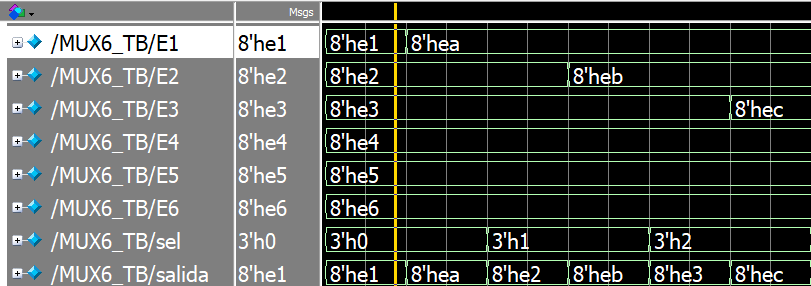
\includegraphics[width=\columnwidth]{Sim_res1_6.png}
		\caption{Resultados de la simulación (Parte 1).}
		\label{fig:MUX6_SIM_RES:1a}
	\end{subfigure}
	
	\vspace{0.5cm} % Espacio vertical entre las subfiguras
	
	% Segunda subfigura
	\begin{subfigure}[b]{\columnwidth}
		\centering
		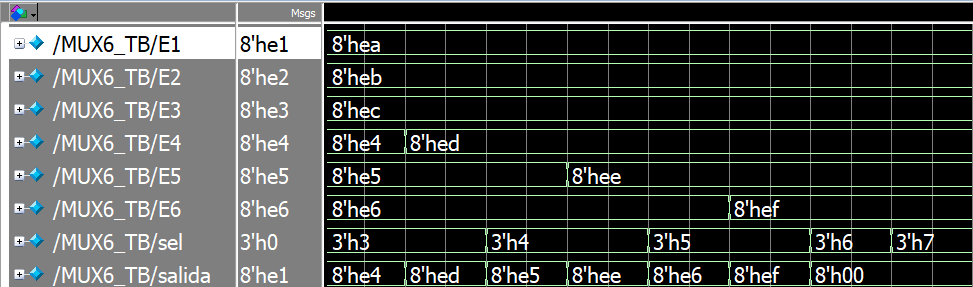
\includegraphics[width=\columnwidth]{Sim_res7_14.png}
		\caption{Resultados de la simulación (Parte 2).}
		\label{fig:MUX6_SIM_RES:1b}
	\end{subfigure}
	
	\caption{Resultados obtenidos tras la simulación del MUX 6:1.}
	\label{fig:MUX6_SIM_RES:1}
	\end{figure}

	Como se muestra en la figura \ref{fig:MUX6_SIM_RES:1a}, cuando el selector (sel) toma el valor de $3'b000$, se selecciona la primera entrada (E1), y es este valor el que se refleja en la salida. Al cambiar el valor de la entrada E1, el valor de la salida también cambia de manera correspondiente. Lo mismo ocurre con el resto de las entradas; al cambiar el valor del selector a $3'b001$, la salida toma el valor de la entrada E2, y al modificar el valor de la entrada seleccionada, la salida se actualiza en consecuencia.



	\section*{Conclusiones}
	La verificación de circuitos digitales es fundamental para asegurar el correcto funcionamiento de un circuito lógico. Utilizando las herramientas de Questasim, se logró diseñar y verificar un multiplexor de 6 entradas y 1 salida de 8 bits. Los resultados obtenidos confirman que el diseño del multiplexor es correcto y que su funcionamiento cumple con las expectativas, asegurando que los casos críticos están adecuadamente cubiertos y operan de manera adecuada.	


	
	
	\bibliographystyle{IEEEtran}
	\bibliography{References}
	
\end{document}
